%!TEX root = ./main.tex
\documentclass[conference]{IEEEtran}
\IEEEoverridecommandlockouts
% The preceding line is only needed to identify funding in the first footnote. If that is unneeded, please comment it out.
\usepackage{cite}
\usepackage{amsmath,amssymb,amsfonts}
\usepackage{algorithmic}
\usepackage{graphicx}
\usepackage{textcomp}
\usepackage{xcolor}
\usepackage[utf8]{inputenc}
\usepackage{array}
\usepackage{gensymb}
\usepackage{mathtools}
\usepackage{units}
\usepackage{esvect}
\usepackage{multirow}
\usepackage{tikz}
\usepackage{subfig}
\usepackage{url}
\usepackage{listings}

\newcommand{\code}{\texttt}

\DeclarePairedDelimiter\ceil{\lceil}{\rceil}
\DeclarePairedDelimiter\floor{\lfloor}{\rfloor}

\def\BibTeX{{\rm B\kern-.05em{\sc i\kern-.025em b}\kern-.08em
    T\kern-.1667em\lower.7ex\hbox{E}\kern-.125emX}}
\begin{document}

\title{globaleventprognosis}

\author{\IEEEauthorblockN{Phillip Ginter}
\IEEEauthorblockA{\textit{Informatik (IN)} \\
\textit{Hochschule Furtwangen}\\
78120 Furtwangen, Deutschland \\
phillip.ginter@hs-furtwangen.de}
\and
\IEEEauthorblockN{Daniel Schönle}
\IEEEauthorblockA{\textit{Informatik (IN)} \\
\textit{Hochschule Furtwangen}\\
78120 Furtwangen, Deutschland \\
daniel.schoenle@hs-furtwangen.de}
}

\maketitle

% INPUT Content sections
%!TEX root = ./../main.tex
\begin{abstract}
Die freie Online-Enzyklopädie Wikipedia umfasst über 74 Millionen Artikel, die dauerhaft Änderungen unterzogen sind.
Auslöser für diese Änderungen können vielfältig sein. Ereignisse der realen Welt wie z.\,B. die Wahl des deutschen Bundeskanzlers
    führen zu einem starken kurzzeitigen Anstieg der Änderungen an dem entsprechenden Wikipedia-Artikel. Das Ziel dieser Arbeit
ist die Erkennung von Ereignissen der realen Welt, anhand von Änderungen an Wikipedia-Artikeln.
Für die Überwachung und Analyse der Änderung an Wikipedia-Artikeln wird eine Streaming-Data-Architektur entworfen und prototypisch umgesetzt.
    Die Modellierung von Mustern liefert dabei nicht die gewünschten Ergebnisse, weshalb der Einsatz eines Burst-Detection-Algorithmus vorgezogen wird.
TODO: Ziel erreicht, fehlt noch?
\end{abstract}

\begin{IEEEkeywords}
wikipedia, prognosis, global event
\end{IEEEkeywords}
%!TEX root = ./../main.tex
\section{Einleitung}
Wikipedia ist eine freie Online-Enzyklopädie, mit dem Ziel „eine frei lizenzierte und hochwertige Enzyklopädie zu schaffen und damit lexikalisches Wissen zu verbreiten“ \cite{wales.}. Sie umfasst 74 Millionen Artikel, die von eine Commuity von 137.571 Nutzer erstellt und geprüft wurden. Seit 2001 wurden die Artikel 877.073.914 mal editiert, dies entspricht etwa 4.000.000 Edit pro Monat. \cite{wikistat}.
TODO
Aufgrund des kollaborativen Erstellungsprozesses können \cite{wikipedia.}

TODO
Aufgabenstellung hier wiedergeben

\begin{itemize}
    \item Was ist Wikipedia?
    \item Wie viele Artikel, Edits, Autoren hat Wikipedia?\footnote{https://en.wikipedia.org/wiki/Wikipedia:Statistics}
    \item Ein Edit bzw. Update in Wikipedia wird durch ein neues Ereignis der realen Welt ausgelöst. Das kann eine Wahl,
    ein Unfall, politische Konflikte oder eine Sportveranstaltung sein \cite{10.1007978-3-642-36973-5_22}.
    \item Aufgabenstellung
    \begin{itemize}
        \item Für eine Entität (z. B. eine Person des öffentlichen Lebens) aus der Gesamtheite der Wikipedia-Edit-Events in "Echtzeit"
        Events der realen Welt ableiten.
        \item Wir betrachten nur die Metadaten (Zeitstempel, Autor, ...) und nicht den Inhalt der Änderung Änderung (z. B. textuelle Änderung).
        \item ...
    \end{itemize}
    \item Wie sieht so ein Burst of Wikipedia-Edits aus \ref{fig:donald_rumsfelds_resignation_burst}?
\end{itemize}


\begin{figure}[h]
    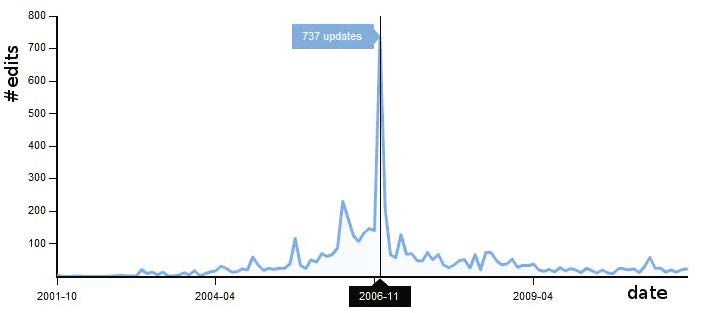
\includegraphics[width=.5\textwidth]{images/Extracting_EventRelated_Information_from_Article.jpg}
    \caption{Donald Rumsfeld’s Rücktritt führte zu einem Burst an Autoren, die einen Wikipedia-Edit vornahmen \cite{10.1007978-3-642-36973-5_22}.}
    \label{fig:donald_rumsfelds_resignation_burst}
\end{figure}
%!TEX root = ./../main.tex
\section{Streaming Data}
Folgendes könnte man in diesem Kapitel behandeln:

\begin{itemize}
    \item Wie sieht eine Streaming Data-Architektur aus bzw. aus welchen Komponenten besteht sie \cite{psaltis2017streaming}?
    \item Ist eine Streaming Data-Architektur für unsere Aufgabenstellung sinnvoll?
    \item Falls ja. Wie ist unsere konkrete Streaming Data-Architektur aufgebaut und wieso?
\end{itemize}



\subsection{Streaming Data-Architektur}
Punkt 1 und 2 von der obigen Liste hier beschreiben mit \cite{psaltis2017streaming}.



\subsection{Konkrete Implementierung unserer Streaming Data-Architektur}
Die obigen vier Stufen einer Streaming Data-Architektur von Psaltis \cite{psaltis2017streaming}
haben wir mit den folgenden konkreten Inhalten gefüllt, um die Aufgabenstellung aus dem vorhergehenden Kapitel zu erfüllen.
In diesem Kapitel geht es um die Frage, wieso wir uns für konkrete Technologien entschieden haben und im nachfolgenden Kapitel
geht es um die Implementierungsdetails dieser Technologien.
\begin{itemize}
    \item \textit{Collection tier.} Wikipedia ist unsere Datenquelle.
    \item \textit{Messaging queuing tier.} Wir nutzen ein Kafka-System: Weshalb Kafka? Welche Features
        (Durable messaging, Different Messaging Systems, Scalability, Performance, Transaction Support, Security, ...) sind für uns von großer Relevanz?
        Oder soll Kafka ein eigenes Kapitel bekommen?
    \item \textit{Analysis tier.} Esper: warum / welche Features sind für uns von Relevanz? Wie sieht die Ausgabe nach der Analyse aus?
    \item \textit{Data access tier.} ???
\end{itemize}
%!TEX root = ./../main.tex
\section{Prototyp}
Zur Lösung der Aufgabenstellung haben wir einen lauffähigen Prototyp entwickelt, der die Machbarkeit demonstriert.
Dafür haben wir die im vorhergehenden Kapitel genannten Technologien eingesetzt. Die Details zu den entstandenen
Anwendungen stellen wir in diesem Kapitel vor.

TODO: Bild der Architektur hier!

\subsection{Collection Tier: Wikipedia}
\begin{itemize}
    \item Was für Daten nutzen wir? WikipediaEditEvents
    \item Welche konkreten Daten hat ein WikipediaEditEvent?
    \item Wie sieht das System dahinter aus; wie verarbeitet Wikipedia die Daten: Kafka
    \item Was ist EventSource und was bringt es hier?
\end{itemize}

\subsection{Implementierungsdetails zum Messaging queuing tier: Kafka}
Im Messaging Queuing Tier setzen wir Apache Kafka in der Version 2.1 ein, um die Wikipedia-Events aus dem Collection Tier
in unser eigenes Messaging-System zu überführen. In der Java-Anwendung werden die folgenden
Schritte nacheinander ausgeführt:
\begin{enumerate}
    \item \textit{Kafka Initialisierung.} Den Host des Bootstrap-Servers setzen. Als Key- und Value-Serialisierer setzen wir
    jeweils den \code{StringSerializer} von Kafka ein. Das heißt, die Events werden als JSON-String in das Topic \code{wikiEdit}
    eingespeist. Zum Senden von Events erzeugen wir ein Producer-Objekt mit dem passenden Typ \code{Producer<String, String>}.
    TODO: Vor- und Nachteile für eine De-/Serialisierung von der eigenen WikipediaEditEvent-Klasse diskutieren
    \item \textit{Erzeugung eines EventHandlers.} Für das Empfangen von EventSource-Nachrichten nutzen wir die Java-Bibliothek
    \textit{okhttp-eventsource}\footnote{https://github.com/launchdarkly/okhttp-eventsource}. Zur Verarbeitung der Events
    \code{onOpen}, \code{onClose}, \code{onMessage}, \code{onComment} und \code{onError} muss das Interface \code{EventHandler} von
    \textit{okhttp-eventsource} implementiert werden.
    \item \textit{Erzeugung und Starten einer EventSource.} Mit der Stream-URI der Wikipedia-EventSource und des implementierten EventHandler-Interfaces
    kann ein \code{EventSource}-Objekt erzeugt werden. Das Objekt dient dem Starten und Beenden eines EventSource-Streams.
    \item \textit{Beim Eintreffen eines Events, Senden einer Nachricht in ein Kafka-Topic.} Tritt ein Wikipedia-Event auf,
    wird die \code{onMessage}-Methode des implementierten EventHandlers-Interface aufgerufen. Einer der beiden Parameter enthält die Daten
    des aufgetretenen Events. Der Zugriff auf die als JSON-String codierte Nachricht erfolgt über die \code{getDate()}-Methode.
    Diese Daten sendet die Anwendung, über den zuvor erzeugten Producer, in das Kafka-Topic \code{wikiEdit}.
\end{enumerate}

Zusammenfassung:
- Die Konfiguration von Kafka: Welche Topics gibt es? Partitionen? Consumer Groups? Replication? Persistence? (oder alles schon im vorherigen Kapitel schreiben)
TODO:
- Vor- und Nachteile für eine De-/Serialisierung von der eigenen WikipediaEditEvent-Klasse diskutieren und der Einsatz von GSON?

\subsection{Implementierungsdetails zum Analysis tier: Esper}
In unserer Esper-Anwendung des Analysis Tier, nutzen wir Esper als Complex Event Processing-Werkzeug. Zur Verarbeitung
der Wikipedia-Events haben wir die folgenden Schritte implementiert:

Genaueres zu den erzeugten Expressions im nächsten Kapitel.

\begin{enumerate}
    \item \textit{Esper Initialisierung.} Die Initialisierung von Esper besteht
    \item \textit{Expression erzeugen.}
    \item \textit{\code{UpdateListener} implementieren.}
    \item \textit{Kafka initialisieren.}
    \item \textit{Kafka Consumer erzeugen und in Endlosschleife Events pollen.}
    \item \textit{Empfangene Events auswerten.}
\end{enumerate}
\section{Analyse}
\begin{itemize}
    \item Welche Expressions nutzen wir?
    \item Wie sind wir auf die Expressions gekommen? Nur durch ausprobieren?
    \item Reale Beispiele für "passende" Events
    \item Welche neuen "Komplexen Events" erzeugen wir?
    \item Reale Beispiele für komplexe Events
    \item Welche Ergebnisse liefert das System?
\end{itemize}
%!TEX root = ./../main.tex
\section{Ergebnisse}

\section{Diskussion}
aa
\section{Ausblick}

\section{Beiträge der Autoren}
 Phillip und Daniel Schönle haben gleichermaßen zu dieser Arbeit beigetragen und sind Erstautoren.

% Quellenverzeichnis
\bibliographystyle{IEEEtran}
\bibliography{bibtex}

\end{document}
